\documentclass{standalone}
\usepackage{tikz}
\standaloneconfig{margin=0pt}

\definecolor{c1}{HTML}{CAD6E9}
\definecolor{c12}{HTML}{99AAC5}
\definecolor{c13}{HTML}{687FA0}
\definecolor{c2}{HTML}{37537C}
\definecolor{c3}{HTML}{86a86c}
\definecolor{c4}{HTML}{6f8dbc}
\definecolor{c5}{HTML}{896190}
\definecolor{c6}{HTML}{B2746B}
\definecolor{c7}{HTML}{CFA08C}
\definecolor{c8}{HTML}{EBCDAD}
\def\xone{3.7}
\def\xthree{5.4}
\def\xtwo{7.45}
\def\xfour{10.6}
\def\xfive{11.9}
\def\xsix{13.2}
\def\xseven{1.87}
\def\xeight{0.3}
\def\xnine{0.9}
\def\y{-0.38}
\begin{document}

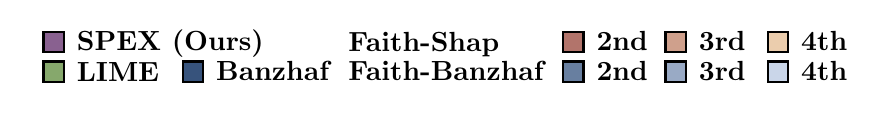
\begin{tikzpicture}
\useasboundingbox (4.0,-.3) rectangle (14.45,.45);
    % Draw SpectralExplain Soft box
    \draw[fill=c5, thick] (.2+\xone+\xeight,0.4) rectangle (0.46+\xone+\xeight,0.14);
    \node[anchor=west] at (0.5+\xone+\xeight,0.25) {\textbf{SPEX (Ours)}};

    \draw[fill=c3, thick] (.2+\xone+\xeight,0.4+\y) rectangle (0.46+\xone+\xeight,0.14+\y);
    \node[anchor=west] at (0.5+\xone+\xeight,0.27+\y) {\textbf{LIME}};

    \draw[fill=c2, thick] (.2+\xone+\xseven-1+\xeight+\xnine,0.4+\y) rectangle (0.46+\xone+\xseven-1+\xeight+\xnine,0.14+\y);
    \node[anchor=west] at (0.5+\xone+\xseven-1+\xeight+\xnine,0.28+\y) {\textbf{Banzhaf}};

    \node[anchor=west] at (0.5+\xtwo,0.28+\y) {\textbf{Faith-Banzhaf}};

    \draw[fill=c13, thick] (.2+\xfour,0.4+\y) rectangle (0.46+\xfour,0.14+\y);
    \node[anchor=west] at (0.5+\xfour,0.28+\y) {\textbf{2nd}};

    \draw[fill=c12, thick] (.2+\xfive,0.4+\y) rectangle (0.46+\xfive,0.14+\y);
    \node[anchor=west] at (0.5+\xfive,0.28+\y) {\textbf{3rd}};

    \draw[fill=c1, thick] (.2+\xsix,0.4+\y) rectangle (0.46+\xsix,0.14+\y);
    \node[anchor=west] at (0.5+\xsix,0.28+\y) {\textbf{4th}};

    \node[anchor=west] at (0.5+\xtwo,0.24) {\textbf{Faith-Shap}};

    \draw[fill=c6, thick] (.2+\xfour,0.4) rectangle (0.46+\xfour,0.14);
    \node[anchor=west] at (0.5+\xfour,0.28) {\textbf{2nd}};

    \draw[fill=c7, thick] (.2+\xfive,0.4) rectangle (0.46+\xfive,0.14);
    \node[anchor=west] at (0.5+\xfive,0.28) {\textbf{3rd}};

    \draw[fill=c8, thick] (.2+\xsix,0.4) rectangle (0.46+\xsix,0.14);
    \node[anchor=west] at (0.5+\xsix,0.28) {\textbf{4th}};

\end{tikzpicture}

\end{document}